\section{Pflichfach}
\subsection{Introduction of Automation Test and Opto-electrical Instrument}
This is a Fachkurs in the first semester, a introductory course. The teacher talks about what is measurement, and measurement that applied in different areas. The main part of the course introduces the graduate schools in our university.

\subsection{Error Theory and Digital Processing}
This course is consist of three parts: error theory, data processing, and uncertainty.
\paragraph{Error} Measurement error($e$) is the difference between a measured value($\hat{x}$) of quantity and its true value($X$). There are two types of measurement error: systematic errors and random errors.

$$e=|\hat{x}-X|$$

If parament $Y$ is acquired by indirect measurement

$$Y=a_1X_1+\dots+a_nX_n$$

then the measurement error of $Y$ is

$$\delta Y=\frac{\partial Y}{\partial X_1}\delta X_1 + \dots + \frac{\partial Y}{\partial X_n}\delta X_n$$

\paragraph{Linear Least Squares} It often happens that $A\mathbf{x}=\mathbf{b}$ has no solution. The usual reason is: too many equations. And this happens in measurement. We can get as much as measurement value as we want, and finally we want a better evaluation from the data we got. Assume we got a evaluation $\mathbf{x}$, then the evaluation error is $e=\mathbf{b} - A \mathbf{x}$. The smaller the error, the better the evaluation. And here comes the least squares.

\subparagraph{Error Equations}
set $v_i$ is the error with measurement value $l_i$, the true value is $f_i(x_1, x_2, \dots, x_t)$, its evaluation $y_i = a_{i1}x_1+a_{i2}x_2+\dots a_{it}x_t$. The error equations is:

\begin{equation*}
\left.
  \begin{array}{lr}
    v_1 = l_1 - y_1, &  \\
    v_2 = l_2 - y_2, & \\
    \dots \\
    v_n = l_n - y_n
  \end{array}
\right\}
\end{equation*}

In matrix form:
\begin{equation*}
  \begin{bmatrix}
    v_1 \\
    v_2 \\
    \vdots \\
    v_n
  \end{bmatrix}
  =
  \begin{bmatrix}
    l_1 \\
    l_2 \\
    \vdots \\
    l_n
  \end{bmatrix}
  -
  \begin{bmatrix}
    a_{11} & a_{12} & \ldots & a_{1t} \\
    a_{21} & a_{22} & \ldots & a_{2t} \\
    \vdots & \vdots & \ddots & \vdots \\
    a_{n1} & a_{n2} & \ldots & a_{nt}
  \end{bmatrix}
  \begin{bmatrix}
    x_1 \\
    x_2 \\
    \vdots \\
    x_t
  \end{bmatrix}
\end{equation*}
which is
\begin{equation} \label{equ_error}
V=L-A\hat{X}
\end{equation}

The object is to minimize the error:
\begin{equation} \label{equ_squ_error}
V^TV=0
\end{equation}

Differentiating equation \ref{equ_squ_error} with respect to x, we get:
$$\textbf{min }A^TV=0$$

Substitute $V$ with equation \ref{equ_error}, we get:
\begin{equation*}\label{equ_lsq}
  (A^TA)\hat{X}=A^TL
\end{equation*}

Thus the optimal evaluation is:
\begin{equation*}
  \hat{X}=(A^TA)^{-1}A^TL
\end{equation*}

\subparagraph{Beispiel}
对三段刻线间距的各种组合量进行了测量,得如下测量数据(单位mm):
$l_1=x,l_2=x,\dots,l_6=x$
试给出这三段刻线间距的最小二乘估计量$x_1,x_2,x_3$及其标准不确定度。
\begin{equation*}
\left.
  \begin{array}{lr}
    v_1 = l_1 - x_1, &  \\
    v_2 = l_2 - x_2, & \\
    v_3 = l_3 - x_3, & \\
    v_4 = l_4 - (x_1+x_2), & \\
    v_5 = l_5 - (x_2+x_3), & \\
    v_6 = l_6 - (x_1+x_2+x_3)
  \end{array}
\right\}
\end{equation*}

\paragraph{Uncertainty} Diese grenzt einen Wertebereich ein, innerhalb dessen der wahre Wert der Messgröße mit einer anzugebenden Wahrscheinlichkeit liegt (üblich sind Bereiche für ungefähr 68 \% und ungefähr 95 \%).

\begin{itemize}
  \item Typ-A: Ermittlung aus der statistischen Analyse mehrerer statistisch unabhängiger Messwerte aus einer Messwiederholung.

  $$u=s=\sqrt{\frac{\sum_{i=1}^{n}v_i^2}{n-1}}$$

  \item Typ-B: Ermittlung ohne statistische Methoden.
\end{itemize}

The combined standard uncertainty of the output quantity $u_C(y)$ can be expressed via the standard uncertainties of the input quantities $u(x_i)$ as follows:
\begin{equation*}
  u_c(y)=\sqrt{[\frac{\partial Y}{\partial X_1} u(X_1)]^2+[\frac{\partial Y}{\partial X_2} u(X_2)]^2+\dots+[\frac{\partial Y}{\partial X_n}u(X_n)]^2}
\end{equation*}

Note that if $X_i$ is random error, then $u(X_i)$ should be multiplied by 1/N additionally.

\subparagraph{erweiterte Unsicherheit} Dieser Kennwert kennzeichnet einen Wertebereich, der den wahren Wert der Messgröße mit hoher Wahrscheinlichkeit enthält.

\subsection{Automatic Test System}
This course introduces several types of bus used in automated electronic test and measurement systems, including PC-DAQ, GPIB/IEEE-488, VXI, PXI, and LXI. The kernel of an ATS lies in Bus interface and Software.

\paragraph{ATS} An ATS is consist of a number of instruments and computer. It can accomplish a certain amount of testing task according to the instructions. The main components of an ATS is:

\begin{enumerate}
  \item instrument controller(typically an PC)
  \item instruction-driven instruments
  \item standard testing bus
  \item software and develop environments
\end{enumerate}

\paragraph{PC-DAQ} \emph{Data acquisition} is the process of sampling signals from the real world and converting the resulting samples into digital numeric values that can be manipulated by a computer.

\paragraph{IEEE-488} IEEE-488 is an 8-bit, electrically parallel bus, with 3 line for handshake(DAV/Data Valid, NRFD/Not Ready for Data, and NDAC/Data Not Accepted). Five lines are used for addressing, and the bus supports up to 31 possible devices, with the cable length of up to 20 metres. The devices are attributed with ``listener'', ``controller'', and ``talker''.

\subparagraph{SCPI} While IEEE-488.1 defines the hardware interface, the software standard still remains blank. And IEEE-488.2 comes with a set of software protocol. And SCPI was introduced as an industry standard, with a set of general commands that each type of devices must obey, which improves software portability.

\paragraph{VXI} VXI is the VMEbus eXtensions for Instrumentation. VXI was introduces as the increasing demand for data rate in testing area. It has more precise timing and synchronization, which improve measurement capability.

\subparagraph{Commander/Servant Hierarchies} The VXIbus defines a Commander/Servant communication protocol so you can construct hierarchical systems using conceptual layers of VXI devices. This structure is like an inverted tree.

All devices has a configuration registers, and the system can identify each VXI device(type, model and manufacturer, address space, and memory requirements). In addition, VXI also defines Message-Based devices, which are required to have communication registers using Word Serial Protocol that is very similar to IEEE 488 protocol.

\subparagraph{VISA} One of the most notable benefits of VISA(\emph{Virtual Instrument Software Architecture}) is its ability to significantly reduce the time and effort involved in programming different I/O interfaces. Instead of using a different API devoted to each interface bus, you can use the VISA API regardless of whether your system is controlled by GPIB, VXI, or a GPIB-VXI. VISA is maintained by VXIplug\&play alliance(VPP).

\subparagraph{IVI} While VISA provides an abstraction of I/O interface(GPIB, VXI, etc), the IVI(Interchangeable Virtual Instrumentation) aims to provide a standard for instrument drivers.

\paragraph{PXI} PXI is based on CompactPCI, and it offers all of the benefits of the PCI architecture including performance, industry adoption.

PXI adds a rugged CompactPCI mechanical form-factor, an industry consortium that defines hardware, electrical, software, power and cooling requirements. Then PXI adds integrated timing and synchronization that is used to route synchronization clocks, and triggers internally.

Most PXI instrument modules are register-based products.

\paragraph{LXI} The LXI Standard defines the communication protocols for instrumentation and data acquisition systems using Ethernet. The LXI Standard has three major elements:
\begin{enumerate}
  \item A standardized LAN interface that provides a framework for web based interfacing and programmatic control.(Type C)
  \item A trigger facility based on the IEEE 1588 Precision Timing Protocol that enables modules to have a sense of time.(Type B)
  \item A physical wired trigger system that tightly synchronizes the operation of multiple LXI instruments.(Type A)
\end{enumerate}

\subsection{Principles of Electronic Measurement}
This course focuses on the fundamentals and structure of electronic instrument. Time/frequency measurement, voltage measurement, the structure of oscilloscope, and frequency spectrum analyzer are covered. Among the items above, time/frequency measurement is the most significant technique, because all the rest technique directly or indirectly involved timing.

\subsubsection{Measuring Time/Frequency}

Time/Frequency measurement has the highest accuracy among others, and time is one of the most basic physical parameters. By definition, period and frequency has the following relationship:
$$f=\frac{1}{T}$$
\paragraph{Frequency} The input signal is initially conditioned to a form that is compatible with the internal circuitry of the counter. The conditioned signal appearing at the door of the main gate is a pulse train where each pulse corresponds to one cycle or event of the input signal. With the main gate open, pulses are allowed to pass through and get totalized by the counting register. The time between the opening to the closing of the main gate or gate time is controlled by the Time Base.

\begin{figure}
  \centering
  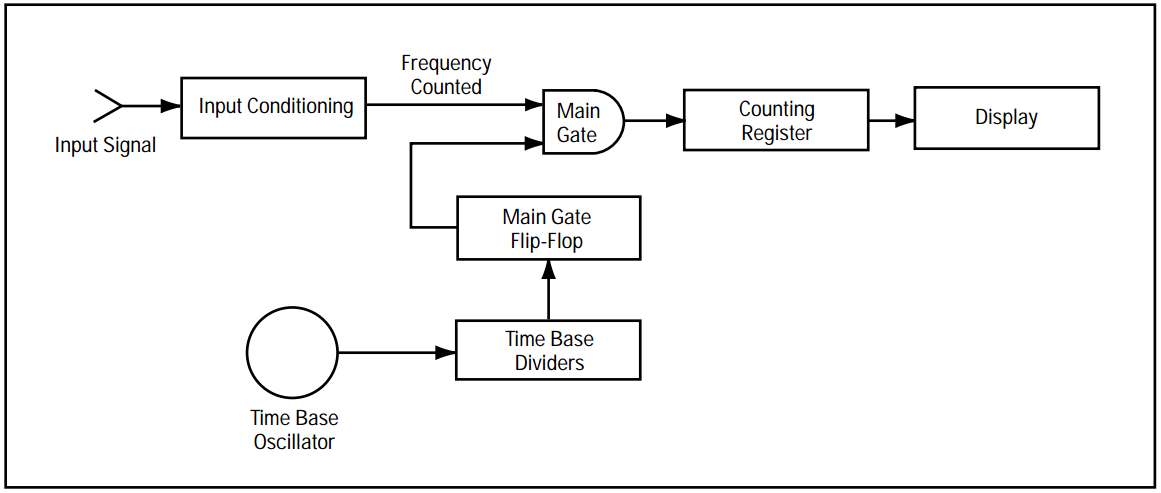
\includegraphics[width=4.5in]{fig/freq_counter.png}
  \caption{Basic block diagram of the conventional counter in its frequency mode of measurement}\label{fig_freq_counter}
\end{figure}

In a specified period $T$, the counter has its value of $N$, then by definition of the frequency, we get

$$f=\frac{N}{T}$$

\paragraph{Time} If we switch the port where frequency signal and time base signal are fed, then the frequency counter can be used for time measurement. By definition:

$$T=\frac{N}{f}$$
where $f$ is the frequency of time base signal.

\subsubsection{Measuring Voltage}

Voltage measurement is more important than other parameters, because others, such as current, power, temperature, pressure, can be converted to voltage.
For an alternating current, it is rectified and measured for RMS value by its \emph{average value} or \emph{peak value}. And the voltage meter presume that the signal is a sinusoidal signal. While peak envelope voltage meter has wider broadband(\SI{1000}{\mega\hertz}), average voltage has better sensitivity.

\begin{itemize}
  \item by converting to direct current

  Peak envelope value, or average value, or root-mean-square value can be converted to direct current.

  \item by calculating with mathematical calculation

  the analog voltage can be converted to digital signal by AD converter, which is easier to couple with.
\end{itemize}

\paragraph{Why RMS?} The purpose of RMS value is to \textbf{simplify power calculations} by providing equivalent DC voltage that would develop the same average power in resistive load.

\paragraph{Crest Factor} crest factor = |peak value| / rms value

\begin{figure}
  \centering
  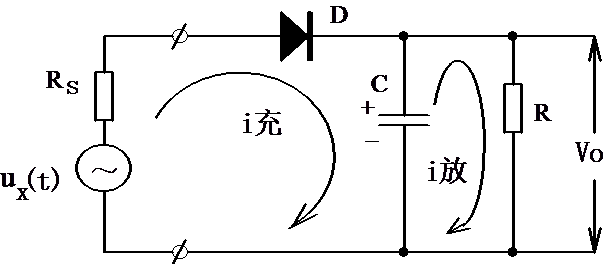
\includegraphics[width=3.0in]{fig/fig_envelop_detector.png}
  \caption{Envelop Detector}\label{fig_envelop_detector}
\end{figure}

The crest factor for a sinusoidal current waveform is 1.414.

\paragraph{Form Factor} form factor = rms value / |average value|

The form factor for a sinusoidal current waveform is 0.9.

\begin{figure}
  \centering
  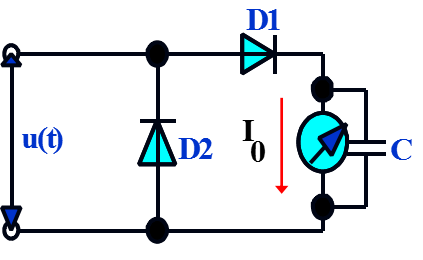
\includegraphics[width=2.5in]{fig/fig_rectified_voltmeter.png}
  \caption{Half Wave Rectifier Circuit for Average value Voltagemeter}\label{fig_rectified_voltagemeter}
\end{figure}

As shown in figure \ref{fig_rectified_voltagemeter}, the rectified voltage is then measured by a gauge.

\subsubsection{Structure of Oscilloscope}
The cathode-ray oscilloscope (C.R.O.) consists of the following components:
\begin{enumerate}
  \item Electron Gun
  \item Deflection System
  \item Display Screen
\end{enumerate}

\begin{figure}
  \centering
  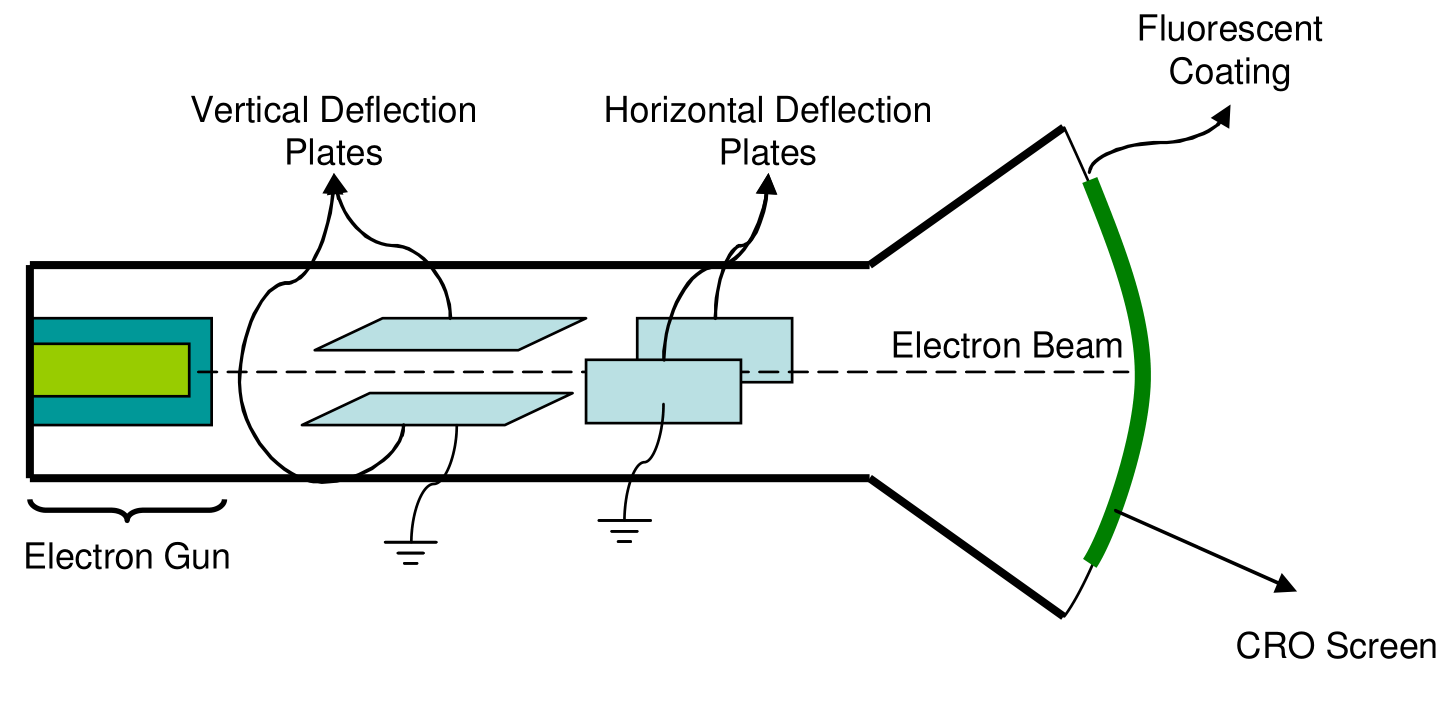
\includegraphics[width=4.5in]{fig/fig_cro.png}
  \caption{Structure Of Cathode Ray Oscilloscope}\label{fig_crc}
\end{figure}

The electron gun generates electron beam, and deflected by the deflection system controlled by X input(horizonal) and Y input(vertical).

Y input is fed by signal to be measured, it may be amplified/attenuated, delayed in the Y channel. The structure of X channel is far more complicate than Y channel. The X channel should generate a signal that is proportional to time(sweeping), when new signal comes at Y channel(trigger).

\paragraph{Pulse generator} The trigger in X channel should generate a pulse to start sweeping circuit when the Y input reaches a certain voltage level(trigger voltage). A pulse may be trigged during sweep cycle, and it should be neglected.

\paragraph{Sweep generator} The sweep generator should produce one cycle of a sawtooth waveform, when it receives a pulse at its input. The period of a sawtooth waveform can be decomposed to two stage: trace stage and flyback stage, as shown in figure \ref{fig_X_channel}.

\begin{figure}
  \centering
  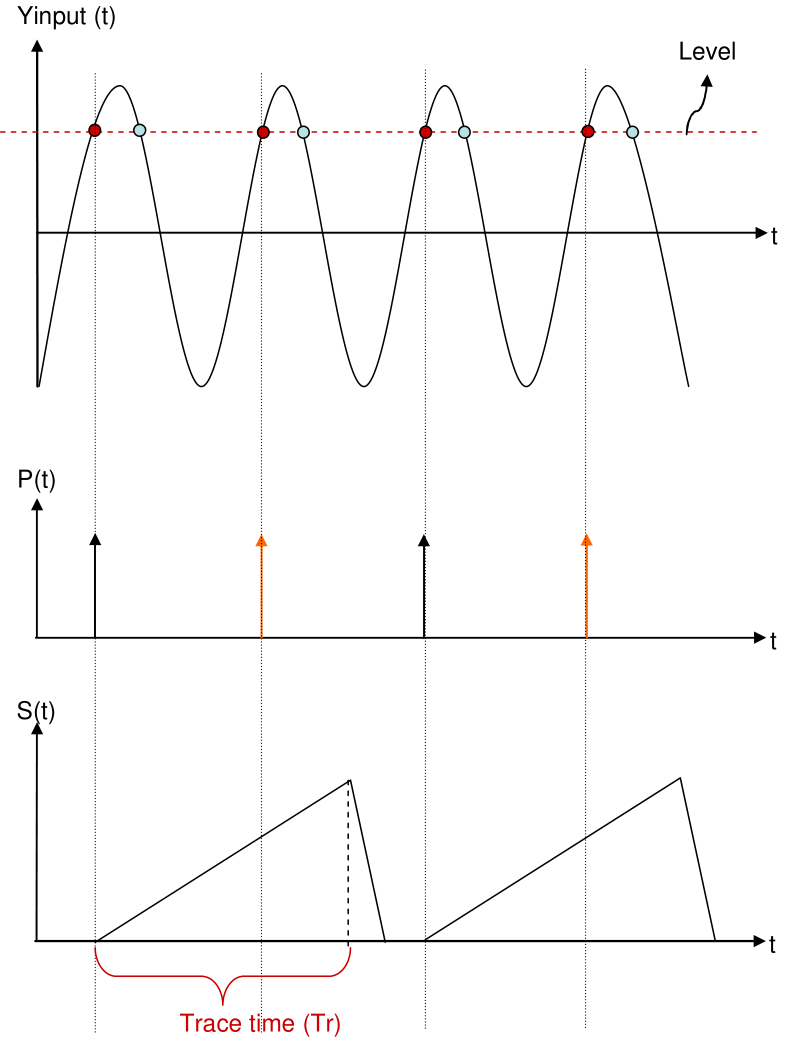
\includegraphics[width=4.2in]{fig/fig_X_channel.png}
  \caption{Sawtooth waveform in X channel}\label{fig_X_channel}
\end{figure}

\subsubsection{Structure of Frequency Spectrum Analyzer}

There are two ways to display the spectrum of a signal: either by acquiring the envelope or by FFT calculation.

The technical parameters of a frequency spectrum analyzer includes:
\begin{itemize}
  \item input range - the maximum range that the analyzer can measure
  \item span - the range that the analyzer can scan once in a time
  \item frequency resolution - determined by IF filter
  \item sweep time - the time required to perform a scan
  \item phase noise - reflects the short-term frequency stability
\end{itemize}

\paragraph{Superheterodyne Spectrum Analyzer}

\begin{figure}
  \centering
  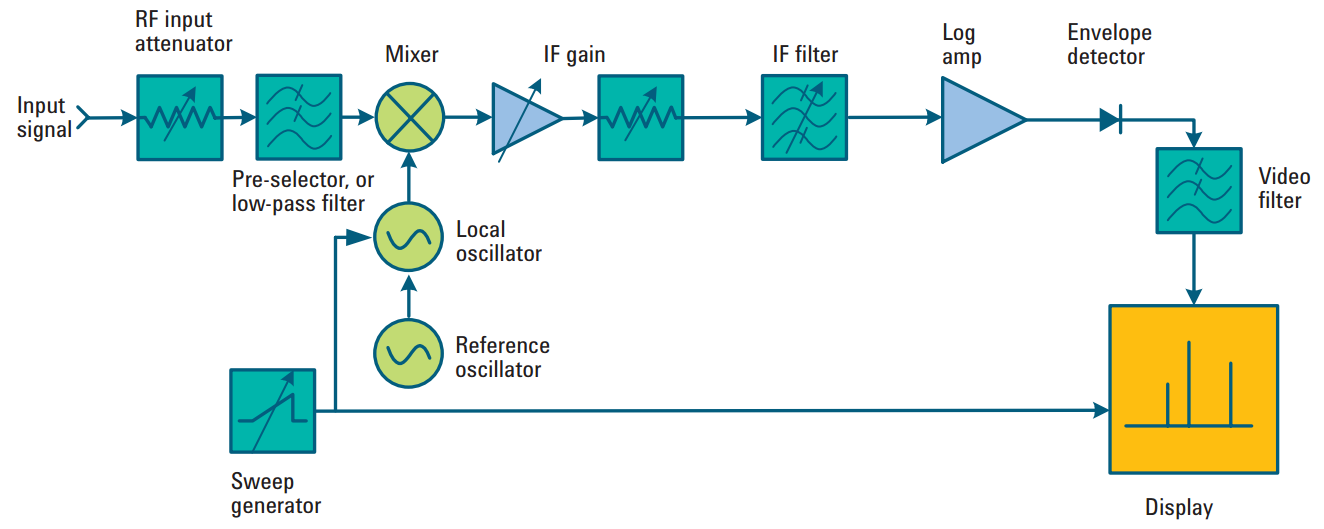
\includegraphics[width=4.5in]{fig/fig_spe_anlyzer.png}
  \caption{Block diagram of a classic superheterodyne spectrum analyzer}\label{fig_spe_anlyzer}
\end{figure}

Figure \ref{fig_spe_anlyzer} is a simplified block diagram of a superheterodyne spectrum analyzer.

\textbf{Heterodyne} means to mix; that is, to translate frequency. And \textbf{super} refers to superaudio frequencies, or frequencies above the audio range.

The input signal passes through an attenuator, then through a low-pass filter to a mixer, and is mixed with a signal from local oscillator(LO). The low-pass filter here is to ease noise from higher frequency, as shown in figure \ref{fig_spectrum_analyser}: $f_L = f_X + f_{IF}$.

\begin{figure}
  \centering
  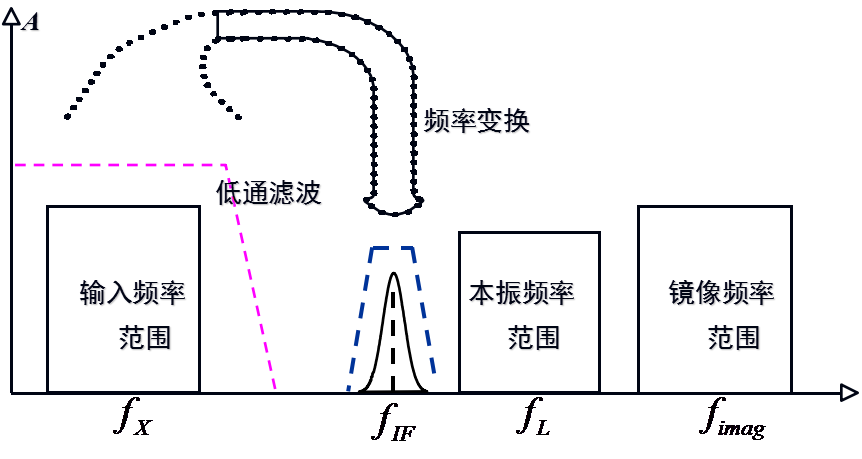
\includegraphics[width=3.5in]{fig/fig_spectrum_analyser.png}
  \caption{the process of spectrum translation}\label{fig_spectrum_analyser}
\end{figure}

It is essentially rectified by the envelope detector, filtered through the low-pass filter and displayed. A ramp generator creates the horizontal movement across the display from left to right. The ramp also tunes the LO so its frequency change is in proportion to the ramp voltage.

\begin{figure}
  \centering
  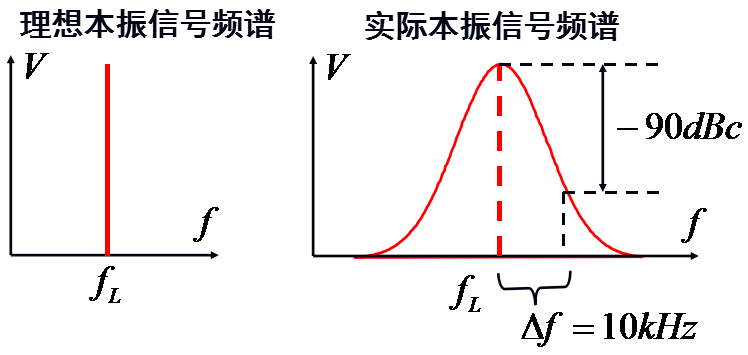
\includegraphics[width=4.2in]{fig/fig_phase_noise.png}
  \caption{Phase noise is displayed only when a signal is displayed far enough above the system noise floor}\label{fig_phase_noise}
\end{figure}

\paragraph{FFT Spectrum Analyzer} The FFT Spectrum Analyzer samples the filtered signal and converts into digital series, then FFT is conducted in microprocessor. It uses digital signal processing techniques to provide in depth waveform analysis with greater flexibility than other methods.

\subsection{Process Control Techniques and Systems}
The main topic of the course is process control system and corresponding control technique.

\subsubsection{Basic Terms}

\paragraph{Process} \emph{Process} refers to the methods of changing or refining raw material(mostly fluid) to create end products.

\paragraph{Process Variable} A \emph{process variable} is a condition that can change the manufacturing process in some way, such as pressure, flow, temperature, pH.

\paragraph{Process control} \emph{Process control} refers to the methods that are used to control process variables(temperature, humidity, etc) when manufacturing a product.

\paragraph{Setpoint} The \emph{setpoint} is a value for a process variable be expected to maintained.

\paragraph{Offset} \emph{Offset} is a sustained deviation from the setpoint.

\subsubsection{Control Loop Components}

There devices that implements the task of measurement, Komparation, and adjustment in the control loop:

\begin{itemize}
  \item sensor
  \item transducer

  A \emph{transducer} is a device that translates a mechanical signal into a electrical signal.

  \item converter

  A \emph{converter} is a device that converts one type of signal into another type of signal, for example \SIrange{4}{20}{\milli\ampere} current signal into another form of pressure signal.

  \item transmitter

  A \emph{transmitter} is a device that converts a signal from sensor/transducer into standard signal and transfers that signal to a monitor or a controller.

  \item indicator
  \item recorder
  \item controller

  A \emph{controller} reads signals from sensor, and output control signal to actuator.

  \item actuator

  An \emph{actuator} is a device that undertakes the task to change the process variables.
\end{itemize}

\subsubsection{Control Algorithms}

\paragraph{PID} The most commonly used control algorithm, P stands for proportional, I stands for integral, and D stands for differential.

\paragraph{Feed forward control} Feed forward control can ease the effect of any disturbance that can be measured.

\paragraph{Smith Predictor} The Smith predictor is a type of predictive controller for systems with \emph{pure time delay}. Subtracting the disturbance-free process variable from the actual process variable yields an \emph{estimate of the disturbances}. By adding this difference to the predicted process variable, Smith created a feedback variable that includes the disturbances, but not the deadtime.

\begin{figure}
  \centering
  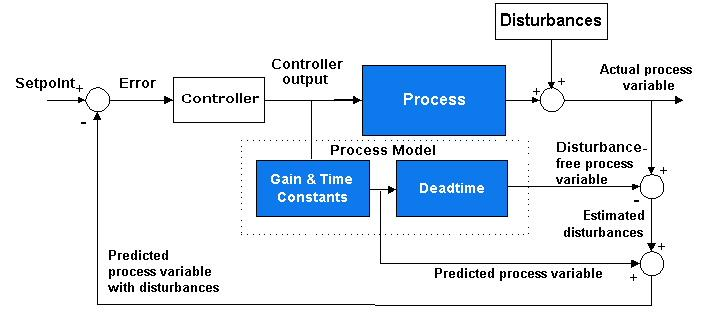
\includegraphics[width=3.5in]{fig/Smith_control2.jpg}
  \caption{Block Diagram of Smith Predictor}\label{fig_smith}
\end{figure}

\subsection{Fundamentals Design of Intelligent Instruments}
This course covers the structure of an instrumentation from microprocessors, Sampling, Human-machine Interfaces, communication interfaces and software developments.

\subsubsection{Sampling}

\begin{figure}
  \centering
  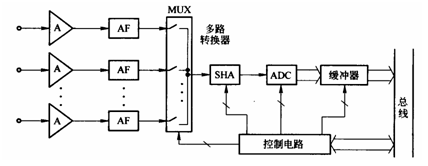
\includegraphics[width=2.5in]{fig/sample_channel.png}
  \caption{Simultaneous Sampling Architecture}\label{fig_sample_channel}
\end{figure}

The structure of a sampling channel is as follows:

\begin{itemize}
  \item multiplexer
  \item sample\& hold circuit
  \item AD converter
\end{itemize}

\paragraph{Signal Conditioning} Input signal may be amplified by front-end amplifier. Front-End amplifiers are mainly used to improve the signal to noise ration at the receiver.

In order to get highest resolution from ADC, the input signal should be amplified in the full range of ADC. The amplifier should have high input impedance, high input bandwidth, high CMRR, low drift, low output noise, and low output impedance.

\begin{figure}
  \centering
  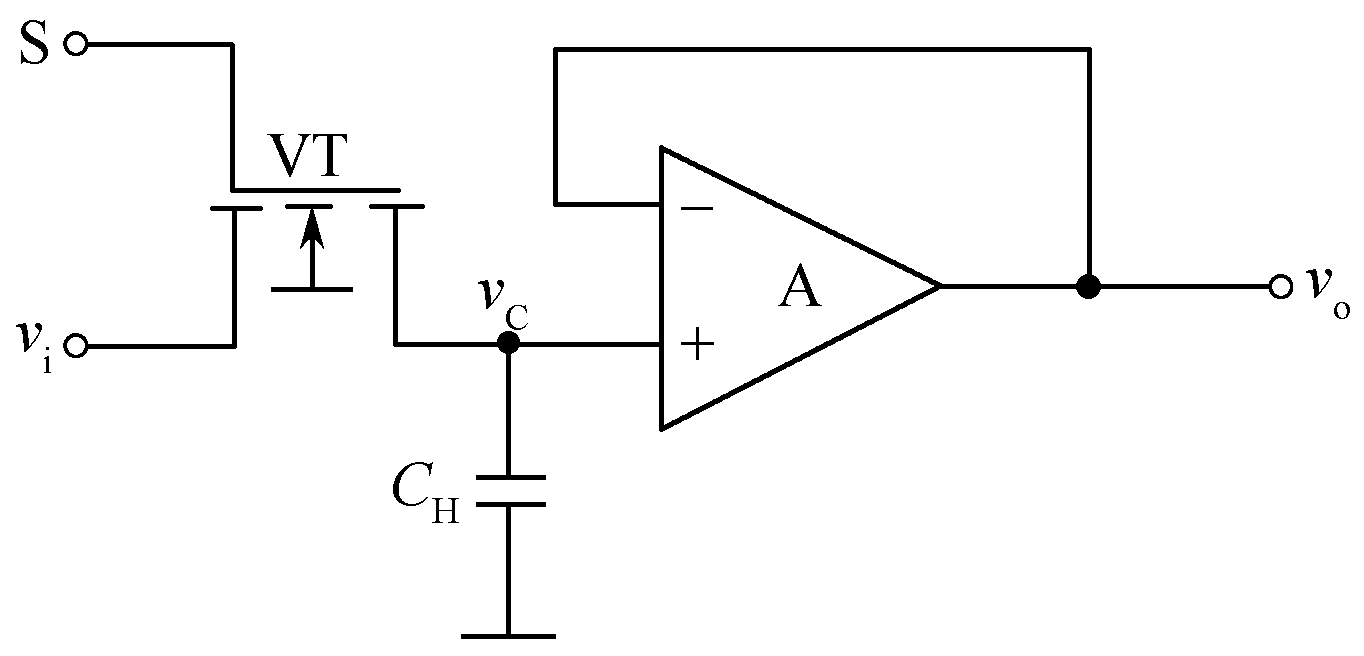
\includegraphics[width=2.5in]{fig/SHA_circuit.png}
  \caption{Sample \& Hold Circuit}\label{fig_SHA}
\end{figure}

\paragraph{AD converter} Three types of AD converter are most applied:

\begin{itemize}
  \item Successive approximation ADC

  low power consumption, high resolution and accuracy, and a small form factor

  \item Slope(integrating) ADC

  high accuracy, low speed, needs external components

  \item $\Sigma - \Delta$ ADC

  high resolution, no calibration needed, no external components

\end{itemize}

\begin{figure}
  \centering
  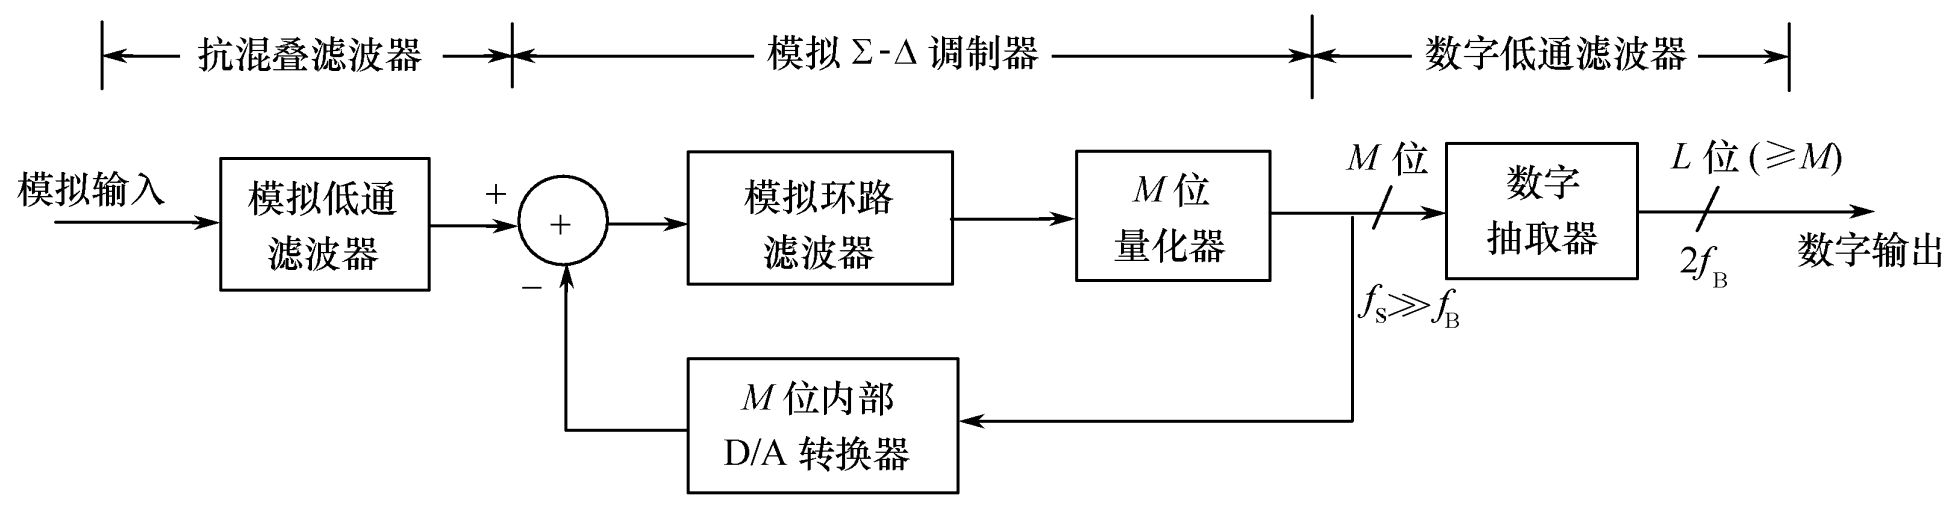
\includegraphics[width=4.5in]{fig/sigma_delta_ADC.png}
  \caption{Sigma-Delta ADC}\label{fig_sigma_delta_ADC}
\end{figure}


\begin{figure}
  \centering
  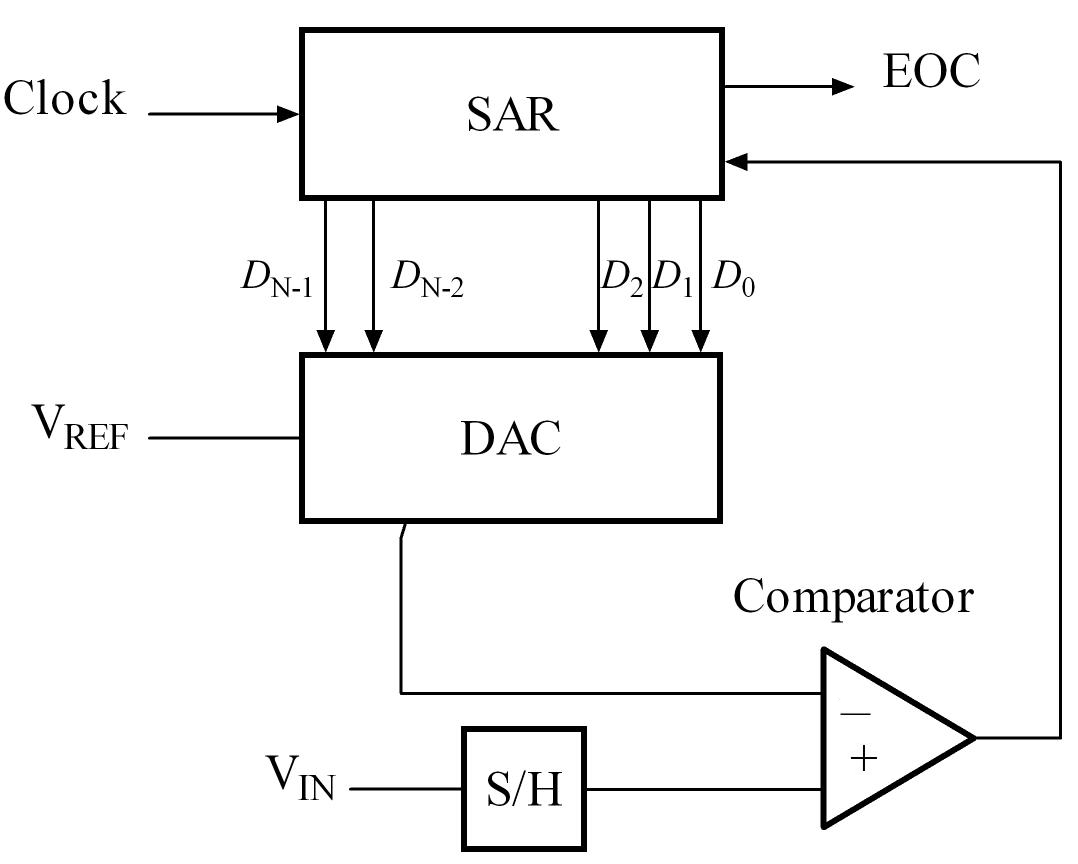
\includegraphics[width=2.5in]{fig/SA_ADC_block_diagram.png}
  \caption{SAR ADC}\label{fig_SAR_ADC}
\end{figure}


\paragraph{Error} Here is a list of errors in the sampling system:
\begin{itemize}
  \item sampling error

  According to Nyquist's theorem, if the signal has frequency of $f_s$, then the sampling system should be $2f_s$ or higher in order to reduce aliasing. So, for an N channel simultaneous sampling system, the minimum frequency required should be $2Nf_s$.

  \item analog circuit error

  Analog circuit error comes from sensor, amplifier, multiplexer, sample \& hold circuit.

  \item ADC error

  Temperature Drift
\end{itemize}

\subsubsection{Human-machine Interface}

Human-machine Interfaces include matrix keypad, LED segment display, and touch screen.

It is important to remove keypad jitter, either by hardware(capacitor) or by software(programmed delay).

\begin{figure}
  \centering
  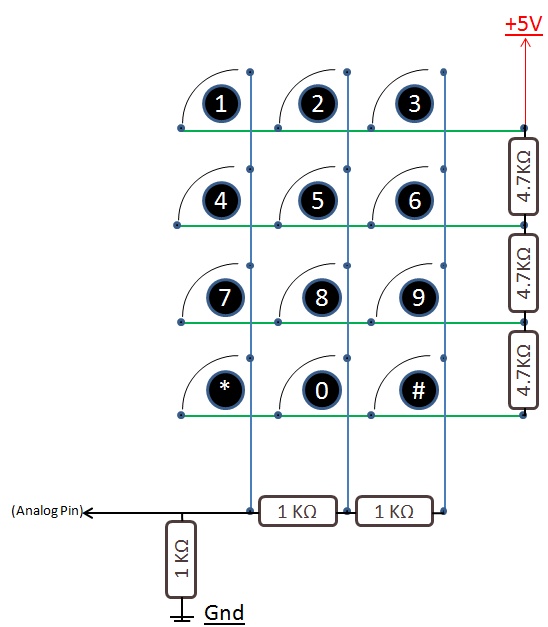
\includegraphics[width=2.2in]{fig/4x3_KeypadLayout.png}
  \caption{4x3 Keypad Layout}\label{fig_keypad}
\end{figure}

If more command are expected than the number of keys on the keypad, then a state machine may be introduced.

\subsubsection{Reliable Software Development}

An instrument may perform self test upon initialization or during runtime, and the content of self test can include circuit, memory(RAM, ROM), bus, keypad, display, etc.

\paragraph{Common Mode Rejection} Common mode rejection may be achieved via following:

\begin{itemize}
  \item differential amplifier
  \item voltage transformer/optical coupling
  \item isolation amplifier
  \item floating ground
\end{itemize}

\subsection{Comprehensive Specialty Experiment}
This is the last course in the university. The students are asked to contact with his/her tutor for a topic to be investigated. My tutor asked me to do a research on the current development of ambient air pollution monitor system and write a review.

\subsubsection{Measurement Component}

\paragraph{Rotatory Encoder} The encoder consists of a light source (LED) and an array of photo-detectors, separated by a slotted disc known as a code wheel. The disc is mounted on the rotating motor shaft. Each time a slot passes between the LED and a detector, the detector receives a flash of light and generates an electrical pulse. 

\subsection{Production Practice}
This is a practical course. The course takes two week: one week in local and the other in Dalian. I paid a visit to several companies, such as Harbin Electric Machinery Company Limited and Dalian Locomotive and Rolling Stock Co., LTD. 